\documentclass[aspectratio=169,11pt]{beamer}

\usepackage{amsmath,amssymb,bm}
\usepackage{booktabs,tabularx,array}
\usepackage{graphicx}
\usepackage{xcolor}

\graphicspath{{docs/presentations/afterSRC-samurai-detector-review/figures/}{../afterSRC-samurai-detector-review/figures/}}

\definecolor{Navy}{HTML}{17324D}
\definecolor{Teal}{HTML}{128C8C}
\definecolor{Gold}{HTML}{D49A2A}
\definecolor{Ink}{HTML}{202A33}
\definecolor{Mist}{HTML}{EEF3F5}
\definecolor{SoftTeal}{HTML}{DDEEEE}
\definecolor{Muted}{HTML}{63717C}

\setbeamercolor{normal text}{fg=Ink,bg=white}
\setbeamercolor{frametitle}{fg=Navy,bg=white}
\setbeamercolor{title}{fg=Navy}
\setbeamercolor{subtitle}{fg=Teal}
\setbeamercolor{structure}{fg=Teal}
\setbeamercolor{alerted text}{fg=Gold}
\setbeamercolor{block title}{fg=white,bg=Navy}
\setbeamercolor{block body}{fg=Ink,bg=Mist}
\setbeamercolor{block title alerted}{fg=white,bg=Teal}
\setbeamercolor{block body alerted}{fg=Ink,bg=SoftTeal}

\setbeamerfont{title}{size=\Huge,series=\bfseries}
\setbeamerfont{subtitle}{size=\Large}
\setbeamerfont{frametitle}{size=\LARGE,series=\bfseries}
\setbeamerfont{block title}{size=\large,series=\bfseries}

\setbeamertemplate{navigation symbols}{}
\setbeamertemplate{frametitle}{\vspace{0.30em}\insertframetitle\par\vspace{0.12em}{\color{Teal}\rule{\textwidth}{1.2pt}}}
\setbeamertemplate{footline}{\leavevmode\hbox to\paperwidth{\hspace{0.65cm}{\color{Muted}\scriptsize\strut SAMURAI73 two-station polarimetry}\hfill{\color{Muted}\scriptsize\strut\insertframenumber/\inserttotalframenumber}\hspace{0.65cm}}\vspace{0.28em}}

\newcommand{\vct}[1]{\bm{#1}}
\newcommand{\Tr}{\operatorname{Tr}}
\newcommand{\Tens}{\bm P^{(2)}}
\newcolumntype{Y}{>{\raggedright\arraybackslash}X}
\newcommand{\conclusion}[1]{\begin{beamercolorbox}[rounded=true,sep=0.55em,wd=\textwidth]{block body alerted}\centering\bfseries\color{Navy}#1\end{beamercolorbox}}

\title{Why SAMURAI73 Needs Two Polarimeters}
\subtitle{Full tensor reconstruction and locating \texorpdfstring{$p_{yy}$}{pyy} loss}
\author{Baiting Tian · Tsinghua University}
\date{3 September 2026}

\begin{document}

\begin{frame}[plain]
  \vspace{1.00cm}
  {\usebeamerfont{title}\color{Navy}\inserttitle\par}
  \vspace{0.45cm}
  {\usebeamerfont{subtitle}\color{Teal}\insertsubtitle\par}
  \vfill
  {\large\color{Ink}\insertauthor\par}
  \vspace{0.25cm}
  {\color{Muted}\insertdate\par}
  \note{[Sources] SAMURAI73 polarized-deuteron IVR proposal; SAMURAI73 polarimeter-location request.}
\end{frame}

% [EN] Open with the operational beam mode and the two locations that bracket the relevant transport. / [CN] 先说明实际束流模式，再用两个位置夹住需要诊断的输运区段。
\begin{frame}{IVR needs the tensor state delivered to the target}
  \centering
  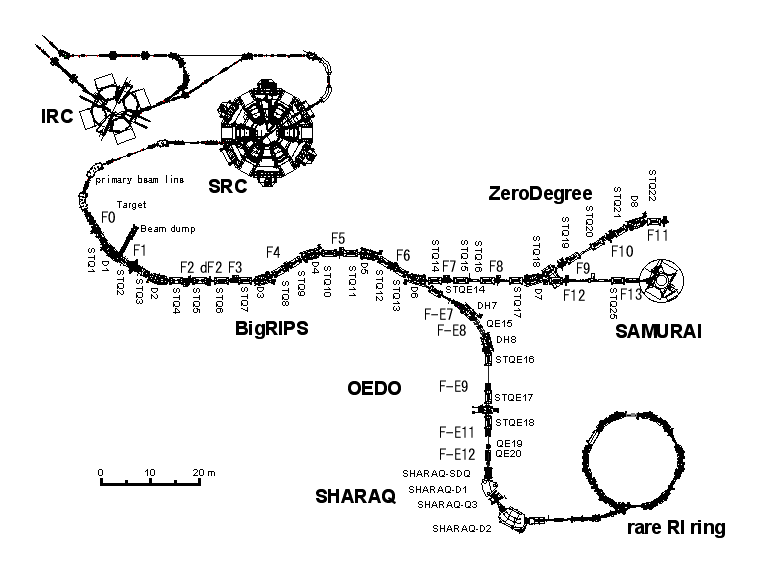
\includegraphics[trim=0 215 0 0,clip,width=0.92\textwidth,height=0.51\textheight,keepaspectratio]{samurai-location-map.png}

  \vspace{0.20em}
  \begin{columns}[T,onlytextwidth]
    \column{0.31\textwidth}
      \textbf{First IVR run}\\[0.15em]
      Start with vertical $p_{yy}$; longitudinal $p_{zz}$ is harder to prepare.
    \column{0.31\textwidth}
      \textbf{After SRC}\\[0.15em]
      What polarization leaves the accelerator chain?
    \column{0.31\textwidth}
      \textbf{After BigRIPS}\\[0.15em]
      What polarization reaches SAMURAI73?
  \end{columns}

  \note{[Sources] RIKEN BigRIPS Technical Information configuration map; SAMURAI73 IVR proposal; user-confirmed plan to begin with pyy because pzz is difficult to prepare.}
\end{frame}

% [EN] Count the full state, tensor-only state, and prepared fixed-axis state without conflating them. / [CN] 分开计算一般态、纯张量态和固定轴制备态的自由度。
\begin{frame}{Spin-1: 8 general degrees, 5 tensor, 1 prepared}
  \begin{columns}[T,onlytextwidth]
    \column{0.47\textwidth}
      For $w_a\geq0$ and $\sum_a w_a=1$,
      \[
        \rho=\sum_a w_a|\psi_a\rangle\langle\psi_a|.
      \]
      A normalized $3\times3$ Hermitian $\rho$ has
      \[
        \boxed{8=3_{\rm vector}+5_{\rm tensor}}
      \]
      independent real parameters.
    \column{0.49\textwidth}
      An axial tensor prepared about $\hat{\vct n}$ is
      \[
        \Tens_0(q,\hat{\vct n})
        =\frac q2\left(3\hat{\vct n}\hat{\vct n}^{\mathsf T}-I\right).
      \]
      \[
        \hat{\vct n}=\hat{\vct y}:
        \quad \Tens_0=\frac{p_{yy}}2\operatorname{diag}(-1,2,-1),
      \]
      \vspace{-0.45em}
      \[
        \hat{\vct n}=\hat{\vct z}:
        \quad \Tens_0=\frac{p_{zz}}2\operatorname{diag}(-1,-1,2).
      \]
  \end{columns}

  \vspace{0.45em}
  \conclusion{Tensor only: 5 degrees. Fixed preparation axis: one amplitude $q$.}
  \note{[Sources] Ohlsen spin-1 density-matrix convention; DPOLAR Cartesian density-matrix parameterization. pyy and pzz are two preparation axes of the same axial-tensor family.}
\end{frame}

% [EN] Separate physical spin evolution from the passive change to the downstream beam basis. / [CN] 将真实自旋演化与下游束流坐标系的被动变换严格分开。
\begin{frame}{Precession is measured in the local beam frame}
  \begin{columns}[T,onlytextwidth]
    \column{0.47\textwidth}
      \textbf{1. Magnetic field rotates the spin in the lab}
      \[
        \rho_{\mathrm{lab},f}
        =U_s\rho_0U_s^\dagger,
        \qquad R_s\in SO(3).
      \]
      Thomas--BMT determines $R_s$ along the trajectory.

    \column{0.47\textwidth}
      \textbf{2. The downstream beam defines new axes}
      \[
        \rho_{b,f}
        =U_o^\dagger\rho_{\mathrm{lab},f}U_o.
      \]
      $R_o$ follows the transported momentum and defines the local $x_b,y_b,z_b$ frame.
  \end{columns}

  \vspace{0.30em}
  \[
    \boxed{R_{\mathrm{rel}}=R_o^{\mathsf T}R_s},
    \qquad
    \Tens_{b,f}=R_{\mathrm{rel}}\Tens_0R_{\mathrm{rel}}^{\mathsf T}.
  \]

  \vspace{0.10em}
  \conclusion{Lowest-order model: one common $R_{\rm rel}$ moves the polarization axis but preserves the tensor eigenvalues and magnitude.}
  \note{[Sources] Thomas-BMT equation; DPOLAR local beam-frame transport convention. The first transformation is physical evolution; the second only re-expresses the same state in the downstream beam basis.}
\end{frame}

% [EN] Treat trajectory-dependent rotation as the higher-order beam effect, not as one unknown rotation. / [CN] 将随轨迹变化的旋转作为高阶束流效应，而不是一个未知旋转。
\begin{frame}{Different trajectories can reduce the ensemble polarization}
  Beyond the central ray, each phase-space point
  $\xi=(x,x',y,y',\Delta p/p,\ldots)$ has its own calculated rotation:
  \[
    \Tens_f(\xi)
    =R_{\mathrm{rel}}(\xi)\Tens_0R_{\mathrm{rel}}^{\mathsf T}(\xi),
    \qquad
    \overline{\Tens}_f
    =\int d\xi\,f(\xi)\Tens_f(\xi).
  \]

  \vspace{0.20em}
  \begin{columns}[T,onlytextwidth]
    \column{0.29\textwidth}
      {\color{Navy}\bfseries 1 degree}\\[0.15em]
      fixed axis and one amplitude $q$
    \column{0.33\textwidth}
      {\color{Navy}\bfseries 3 degrees}\\[0.15em]
      one rigid tensor: $q$ plus two axis angles
    \column{0.33\textwidth}
      {\color{Navy}\bfseries 5 degrees}\\[0.15em]
      a general beam-averaged tensor
  \end{columns}

  \vspace{0.45em}
  {\color{Teal}\bfseries Each particle remains coherent. The average can lose tensor magnitude because the particles arrive with different axes.}
  \note{[Sources] DPOLAR phase-space-averaged spin-transport model. Here ``higher order'' means transport beyond one central trajectory: Rrel varies across the beam phase space.}
\end{frame}

% [EN] Contrast nominal-mode monitoring with model-independent tensor identifiability. / [CN] 区分名义模式监测与不依赖纯模式假设的张量可辨识性。
\begin{frame}{One station sees 4/5 tensor degrees; two see 5/5}
  \begin{columns}[T,onlytextwidth]
    \column{0.47\textwidth}
      \textbf{Nominal $p_{yy}$ monitoring}
      \[
        \frac{N_L+N_R-N_U-N_D}
        {N_L+N_R+N_U+N_D}
        \quad\Longrightarrow\quad p_{yy}.
      \]
      One station measures the amplitude if the beam is assumed to remain a pure $p_{yy}$ state.
    \column{0.47\textwidth}
      \textbf{General-state test}

      One L/R/U/D station is blind to tensor $p_{xy}$ and vector $p_z$.

      \vspace{0.35em}
      A complementary second view rotates these directions into measured combinations.
  \end{columns}

  \vspace{0.45em}
  \renewcommand{\arraystretch}{1.18}
  \begin{tabularx}{\textwidth}{Y c c}
    \toprule
    Calibrated multi-angle measurement & tensor state & full density matrix \\
    \midrule
    one station & $4/5$ & $6/8$ \\
    two stations with characterized complementary transport & $\alert{5/5}$ & $\alert{8/8}$ \\
    \bottomrule
  \end{tabularx}

  \note{[Sources] DPOLAR multi-angle L/R/U/D response and joint-rank analysis. A single tensor station has the exact pxy blind direction; the full response also omits pz.}
\end{frame}

% [EN] Use an axis-independent tensor magnitude to distinguish rotation from loss and the two locations to identify the interval. / [CN] 用与坐标轴无关的张量幅度区分旋转与损失，并用两个位置确定发生区段。
\begin{frame}{Two stations locate a true loss of polarization}
  Use an axis-independent tensor magnitude
  \[
    Q\equiv\sqrt{\frac{2}{3}\Tr\!\left[(\Tens)^2\right]},
    \qquad Q=|p_{yy}|\ \text{for an ideal axial $p_{yy}$ state}.
  \]

  \vspace{0.10em}
  \begin{columns}[T,onlytextwidth]
    \column{0.47\textwidth}
      \textbf{What happened?}

      \vspace{0.20em}
      $Q_2\simeq Q_1$, but the principal axis changes:
      \alert{coherent rotation, not depolarization}.

      \vspace{0.45em}
      $Q_2<Q_1$ after transport correction:
      \alert{true loss of beam-averaged polarization}.
    \column{0.47\textwidth}
      \textbf{Where did the loss occur?}

      \vspace{0.20em}
      $Q_1$ already low after SRC:
      \alert{source, acceleration, or SRC}.

      \vspace{0.45em}
      $Q_1$ nominal, but $Q_2$ low after BigRIPS:
      \alert{between the stations, including BigRIPS transport or acceptance}.
  \end{columns}

  \vspace{0.30em}
  \conclusion{A lower $p_{yy}$ component alone is ambiguous: its axis may have moved, or its magnitude may have fallen.}
  \note{[Sources] Rotation invariance of Tr[(P2)^2]; SAMURAI73 two-station loss-localization requirement. The after-BigRIPS comparison is made against the phase-space-averaged transport prediction.}
\end{frame}

% [EN] End with the concrete coordination decision needed from the RIKEN participants. / [CN] 以需要 RIKEN 参会者确认的具体协调事项收束报告。
\begin{frame}{Who is the contact for an after-SRC polarimeter?}
  \vspace{0.35em}
  {\Large\bfseries\color{Navy}Could a polarimeter be installed just downstream of SRC?\par}

  \vspace{0.75em}
  {\large Who should we contact to discuss\par}
  \vspace{0.30em}
  \begin{itemize}
    \setlength\itemsep{0.45em}
    \item the available beam-line location and longitudinal space;
    \item vacuum, mechanical, electrical, and detector interfaces;
    \item beam optics, operation, radiation safety, and installation constraints?
  \end{itemize}

  \vspace{0.70em}
  \conclusion{Requested next step: identify the responsible beam-line contact and arrange an interface discussion.}
  \note{[Sources] SAMURAI73 polarimeter-location request.}
\end{frame}

\end{document}
